% !TEX root = ../../../main.tex
% 所属：第一部分：单变量分析学 / 第6章：函数的极限与连续性
% 节：6.2 函数极限的性质
% 正文按原文件顺序保存；由 ../chapter6.tex 调用。
\section{函数极限的性质}
下面我们叙述函数极限的性质，我们以\ref{def1}中定义的函数极限为例，而其他的23种极限，在有定义的条件下，可以认为下面的性质同样具备.

\begin{proposition}
	设 $A$ 与 $B$ 都是 $f(x)$ 在 $x_0$ 处的极限，即 $A = B$；换句话说，$f(x)$ 在该点的极限唯一.
\end{proposition}
\begin{proof}
	对 $A$ 与 $B$，由极限的定义，
	$$\begin{aligned}
		\forall \varepsilon > 0, &\exists \delta_1 > 0, \forall x (0 < |x - x_0| < \delta_1): |f(x) - A| < \varepsilon\\
		&\exists \delta_2 > 0, \forall x (0 < |x - x_0| < \delta_2): |f(x) - B| < \varepsilon
	\end{aligned}$$
	取 $\delta = \min\{\delta_1,\delta_2\}$，当 $0 < |x - x_0| < \delta$ 时，
	\[
	|A - B| \leqslant |f(x) - A| + |f(x) - B| < 2\varepsilon
	\]
	因为 $\varepsilon$ 是任意的，所以 $|A - B| = 0$，即 $A = B$.
\end{proof}
函数极限有与数列极限相同 的一条性质(\ref{数列的保序性}).

\begin{proposition}
	设 $\lim\limits_{x \to x_0} f(x) = A$，$\lim\limits_{x \to x_0} g(x) = B$，
	
	若 $A > B$，那么存在 $\delta > 0$，使 $0 < |x - x_0| < \delta$ 时，成立 $f(x) > g(x)$.
	\label{partlimits}
\end{proposition}
\begin{proof}
	$$\begin{aligned}
		\forall \varepsilon > 0,&\exists \delta_1 > 0,\forall x (0 < |x - x_0| < \delta_1): |f(x) - A| < \varepsilon\\
		&\exists \delta_2 > 0,\forall x (0 < |x - x_0| < \delta_2): |g(x) - B| < \varepsilon
	\end{aligned}$$
	取 $\delta = \min\{\delta_1, \delta_2\}$，当 $0 < |x - x_0| < \delta$ 时，以上两式同时成立：
	
	再取 $\varepsilon_0 = \dfrac{A - B}{2}$，$\forall \delta, 0 < |x - x_0| < \delta$：
	
	\[
	g(x) < \frac{A + B}{2} < f(x)
	\]
	
\end{proof}
\begin{corollary}
	1. 若 $\lim\limits_{x \to x_0} f(x) = A \neq 0$，则存在 $\delta > 0$，当 $0 < |x - x_0| < \delta$ 时成立
	\[
	|f(x)| > \frac{|A|}{2}
	\]
	
	2. 若 $\lim\limits_{x \to x_0} f(x) = A$，$\lim\limits_{x \to x_0} g(x) = B$，且 $\exists r > 0$，使 $\forall x (0 < |x - x_0| < r)$ 成立 $g(x) \leqslant f(x)$，则 $B \leqslant A$
\end{corollary}
\begin{proof}
	1. 取 \ref{partlimits}中 $f(x) \Rightarrow |f(x)|$，$g(x) \Rightarrow \dfrac{|A|}{2}$，成立.
	
	2. 若不然，则 $B > A$，由 \ref{partlimits}，$\exists \delta > 0$，$\forall x (0 < |x - x_0| < \delta)$ 成立 $f(x) < g(x)$，
	取 $\eta = \min\{\delta, r\}$，当 $0 < |x - x_0| < \eta$ 时，$f(x) < g(x)$ 与 $g(x) \leqslant f(x)$ 矛盾.
	
\end{proof}
\begin{proposition}
	若 $\lim\limits_{x \to x_0} f(x) = A\in\R$，则存在 $\delta > 0$，使得 $f(x)$ 在 $O(x_0, \delta) \setminus \{x_0\}$ 中有界.
\end{proposition}
\begin{proof}
	取 $\varepsilon = 1$，$\exists \delta > 0$，使 $0 < |x - x_0| < \delta$ 时，$|f(x) - A| < \varepsilon = 1$，
	
	即有
	\[
	A - 1 < f(x) < A + 1 \implies |f(x)| < |A| + 1
	\]
	
	即有界.
\end{proof}
\begin{proposition}
	若存在 $r > 0$，使 $\forall x (0 < |x - x_0| < r)$ 成立 $g(x) \leqslant f(x) \leqslant h(x)$，
	
	且 $\lim\limits_{x \to x_0} g(x) = \lim\limits_{x \to x_0} h(x) = A$，则 $\lim\limits_{x \to x_0} f(x) = A$.
\end{proposition}
\begin{proof}
	$$\begin{aligned}
		\forall \varepsilon > 0,&\exists 0 < \delta_1 < r,\forall x (0 < |x - x_0| < \delta_1): A - \varepsilon < g(x)\\
		&\exists 0 < \delta_2 < r,\forall x (0 < |x - x_0| < \delta_2): h(x) < A + \varepsilon
	\end{aligned}$$
	取 $\delta = \min\{\delta_1, \delta_2\}$，当 $0 < |x - x_0| < \delta$，
	\[
	A - \varepsilon < g(x) \leqslant f(x) <h(x) < A + \varepsilon
	\]
	即
	\[
	|f(x) - A| < \varepsilon
	\]
	$\forall x: 0 < |x - x_0| < \delta$
	\[
	\lim_{x \to x_0} f(x) = A
	\]
\end{proof}
\begin{proposition}
	$$\lim_{x\to0}\frac{\sin x}{x}=1$$
\end{proposition}
\begin{proof}
	$x\to0$且$\dfrac{\sin(-x)}{-x}=\dfrac{\sin x}{x}$，不妨设$0<x<\dfrac{\pi}{2}$
	
	考虑下图
	\begin{center}
		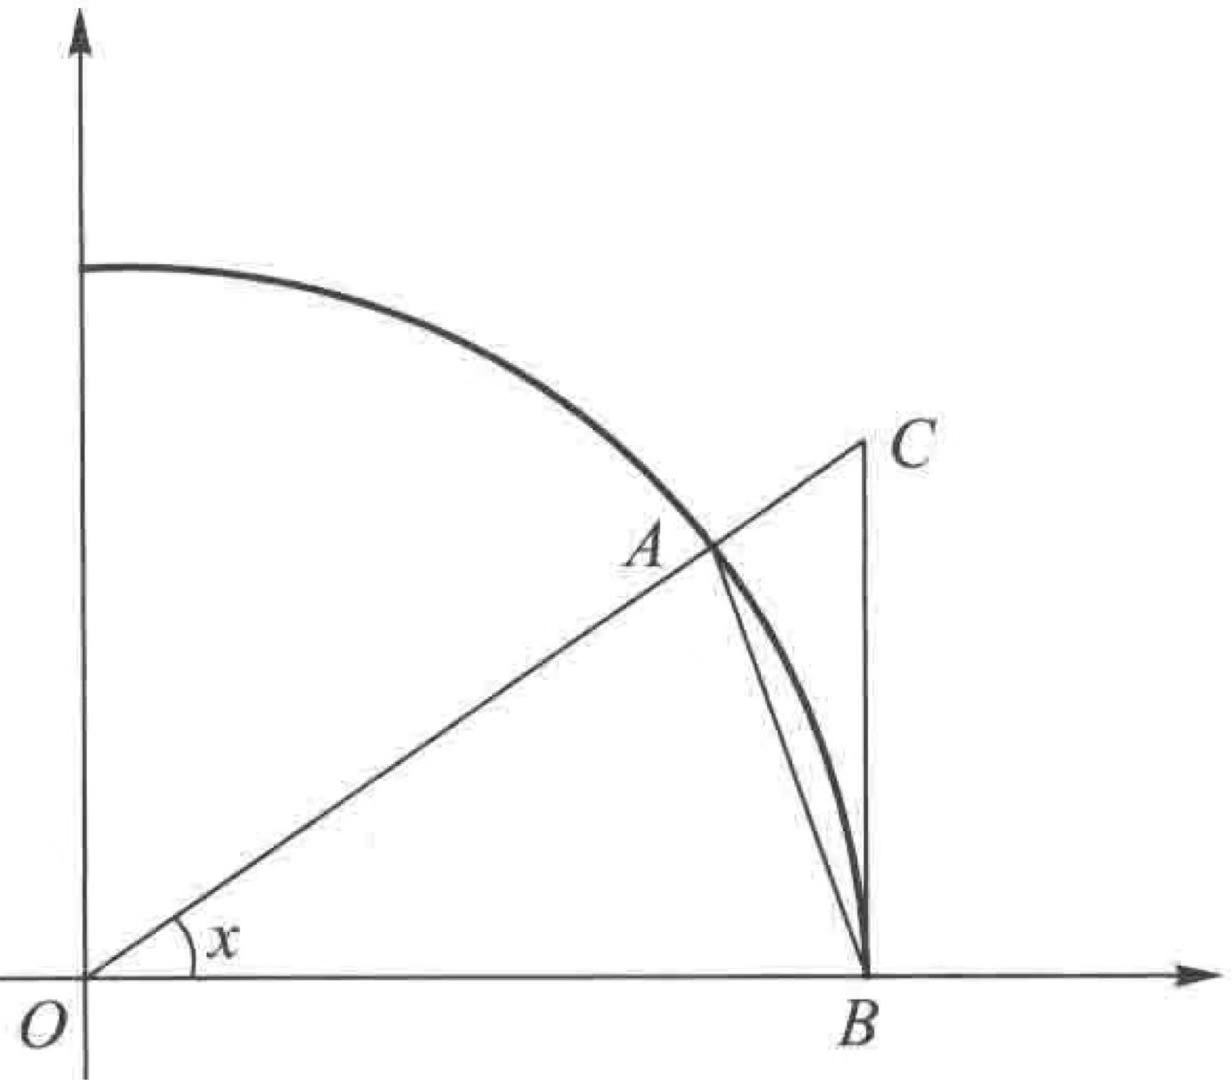
\includegraphics[width=0.3\linewidth]{figure/C5/1}
	\end{center}
	设
	\[
	S_{\triangle OAB} = \frac{1}{2} \sin x = S_1
	\]
	\[
	S_{\triangle OAC} = \frac{1}{2} \tan x = S_2
	\]
	\[
	S_{\textbf{扇形}OAB} = \frac{1}{2} x = S_3
	\]
	
	显然地，
	\[
	S_1 < S_3 < S_2
	\]
	
	也即
	\[
	\sin x < x < \tan x 
	\]
	由于$ x \in \left(0, \dfrac{\pi}{2}\right)$
	\[\frac{\sin x}{x}<1<\frac{\tan x}{x}\Leftrightarrow\cos x<\frac{\sin x}{x}<1\quad x\in(0,\frac{\pi}{2})\]
	下证 $\lim\limits_{x \to 0} \cos x = 1$，也即证明 $f(x) = \cos x$ 在 $x = 0$ 处的连续性.
	
	$\forall \varepsilon > 0$，考虑
	
	\[
	|\cos x - 1| = 2 \sin^2 \frac{x}{2} < \frac{x^2}{2} < \varepsilon
	\]
	
	取 $\delta = \min\left\{\dfrac{\pi}{2}, \sqrt{2\eps}\right\}$，则 $\lim\limits_{x \to 0} \cos x = 1$ 得证.
	
	综上，
	\[
	\lim_{x \to 0} \frac{\sin x}{x} = 1
	\]
\end{proof}
\begin{proposition}
	设 $\lim\limits_{x \to x_0} f(x) = A$，$\lim\limits_{x \to x_0} g(x) = B$，则：
	
	(1) $$\lim_{x \to x_0} (\alpha f(x) + \beta g(x)) = \alpha A + \beta B$$
	
	(2) $$\lim_{x \to x_0} f(x)g(x) = AB$$
	
	(3) $$\lim_{x \to x_0} \frac{f(x)}{g(x)} = \frac{A}{B}\quad B \neq 0$$ 
	
\end{proposition}
\begin{proof}
	$$\begin{aligned}
		\forall \varepsilon > 0,&\exists \delta_1 > 0,\forall x (0 < |x - x_0| < \delta_1): |f(x) - A| < \varepsilon\\
		&\exists \delta_2 > 0,\forall x (0 < |x - x_0| < \delta_2): |g(x) - B| < \varepsilon
	\end{aligned}$$
	
	取 $0 < |x - x_0| < \min\{\delta_1, \delta_2\}$，则两式同时成立.
	
	由有界性：$\forall 0 < |x - x_0| < \min\{\delta_1, \delta_2\}$，$\exists M$，使 $|f(x)| \leqslant M$，$|g(x)| \leqslant M$.
	
	(1)	取 $0 < |x - x_0| < \min\{\delta_1, \delta_2\}$
	\[
	|\alpha f(x) + \beta g(x) - (\alpha A + \beta B)| \leqslant |\alpha||f(x) - A| + |\beta||g(x) - B| < 2\varepsilon
	\]
	
	(2) 取 $0 < |x - x_0| < \min\{\delta_1, \delta_2\}$，
	$$\begin{aligned}
		|f(x)g(x) - AB| &= |f(x)g(x) - g(x)A + g(x)A - AB|\\ 
		&< M|f(x) - A| + |A||g(x) - B| < (M + |A|)\varepsilon
	\end{aligned}$$
	
	
	(3) 取 $0 < |x - x_0| < \min\{\delta_1, \delta_2\}$，
	\[
	\left|\frac{f(x)}{g(x)} - \frac{A}{B}\right| = \left|\frac{Bf(x) - BA + BA - Ag(x)}{Bg(x)}\right| < \frac{2(|A| + |B|)}{B^2} \varepsilon
	\]
	
\end{proof}
\begin{theorem}(Heine定理)\label{Heine1}
	$\lim\limits_{x \to x_0} f(x) = A~\Leftrightarrow~$ $\forall \{x_n\}$ 满足 $x_n \in O(x_0, \rho) \setminus \{x_0\}$ 对某$\rho$，且 $\lim\limits_{n \to \infty} x_n = x_0$，数列 $\{f(x_n)\}$ 满足 $\lim\limits_{n \to \infty} f(x_n) = A$.
\end{theorem}
\begin{proof}
	$\Rightarrow$ 若 $f(x) \to A$ 当 $x \to x_0$，
	
	$\forall \varepsilon > 0, \exists \delta > 0, \forall x (0 < |x - x_0| < \delta): |f(x) - A| < \varepsilon(*)$
	
	由 $x_n \to x_0$，对上述 $\delta > 0, \exists N, \forall n > N$ 
	\[
	0 < |x_n - x_0| < \delta
	\]
	
	由 $(*)$， 因$ x_n \in O(x_0, \rho) \setminus \{x_0\}$，那么 $ |f(x_n) - A| < \varepsilon$
	
	综上$\forall \varepsilon > 0, \exists N, \forall n > N, |f(x_n) - A| < \varepsilon$
	
	$\Leftarrow$ 若不然，$\lim\limits_{x\to x_0}f(x)\neq A$
	
	$\exists \eps_0>0,\forall \delta>0,\exists \widetilde{x},~$即使$0<|\widetilde{x}-x_0|<\delta$，亦有$|f(\widetilde{x})-A|\geqslant\eps_0$
	
	取 $\delta_1 = 1, \exists x_1 (0 < |x_1 - x_0| < \delta_1): |f(x_1) - A| \geqslant \varepsilon_0$，
	
	取 $\delta_2 = \dfrac{1}{2}, \exists x_2 (0 < |x_2 - x_0| < \delta_2): |f(x_2) - A| \geqslant \varepsilon_0$，
	
	$\cdots$
	
	取 $\delta_k = \dfrac{1}{k}, \exists x_k (0 < |x_k - x_0| < \delta_k): |f(x_k) - A| \geqslant \varepsilon_0$，
	
	$\cdots$
	
	这样，我们得到一个列 $\{x_n\}$ 满足 $0 < |x_n - x_0| < \dfrac{1}{n}$ 且 $\lim\limits_{n \to \infty} x_n = x_0$，但是 $|f(x_n) - A| \geqslant \varepsilon_0$，矛盾.
\end{proof}
\begin{corollary}
	(Heine定理的等价叙述)
	$\lim\limits_{x \to x_0} f(x)$ 存在且有限$\Leftrightarrow$对任意序列 $\{x_n\}, x_n \in O(x_0, \rho) \setminus \{x_0\}$ 且 $x_n \to x_0$，$\lim\limits_{n \to \infty} f(x_n)$ 存在且有限.
	
\end{corollary}

\begin{proof}
	必要性$(\Rightarrow)$:同\ref{Heine1}的必要性证明
	
	充分性$(\Leftarrow)$:
	由\ref{Heine1}，只需对任意序列 $\{x_n\}$，$\{f(x_n)\}$ 收敛于同一极限.
	
	如若不然，设 $\{x_n'\}$ 满足 $x_n' \to x_0$，且 $f(x_n') \to A$;$\{x''_n\}$ 满足 $x''_n \to x_0$，且 $f(x''_n) \to B$.
	
	构造数列 $\{x_n\}$ 令 $x_{2n-1} = x_n'$，$x_{2n} = x''_n$，则 $x_n \to x_0$，但 $f(x_n)$ 不收敛，矛盾.
\end{proof}
\begin{example}
	(1) 考虑 $f(x) = \dfrac{a_n x^n + \cdots + a_k x^k}{b_m x^m + \cdots + b_j x^j}$ 在 $x \to 0$ 或 $x \to \infty$ 处的极限.
	
	(2) 证明
	\[
	\lim_{x \to \infty} \left(1 + \frac{1}{x}\right)^x = e
	\]
	
	(3) 证明
	\[
	\lim_{x \to 0} \sin \frac{1}{x} \text{ 不存在}
	\]
\end{example}
\begin{proof}
	(1)
	\[
	\lim_{x \to 0} f(x) =
	\begin{cases}
		\dfrac{a_k}{b_k}, & k = j, \\
		0, & k > j, \\
		\infty, & k < j.
	\end{cases}
	\]
	
	\[
	\lim_{x \to \infty} f(x) =
	\begin{cases}
		\dfrac{a_n}{b_m}, & n = m, \\
		0, & n < m, \\
		\infty, & n > m.
	\end{cases}
	\]
	(2)先考虑$\lim\limits_{x\to+\infty}(1+\dfrac{1}{x})^x$
	
	$\forall x \geqslant 1$，
	\[
	\left(1 + \frac{1}{\lfloor x \rfloor}\right)^{\lfloor x \rfloor} < \left(1 + \frac{1}{x}\right)^x < \left(1 + \frac{1}{\lfloor x \rfloor + 1}\right)^{\lfloor x \rfloor + 1}
	\]
	
	对上式左右两取极限，等价于下式，
	\[
	\lim_{n \to \infty} \left(1 + \frac{1}{n+1}\right)^{n} = e \quad \text{且} \quad \lim_{n \to \infty} \left(1 + \frac{1}{n}\right)^{n+1} = e
	\]
	由夹逼性，
	\[
	\lim_{x \to +\infty} \left(1 + \frac{1}{x}\right)^x = e
	\]
	考虑 $x \to -\infty$ 的情况，令 $y = -x$，$y \to +\infty$，则
	\[
	\lim_{x \to -\infty} \left(1 + \frac{1}{x}\right)^x = \lim_{y \to +\infty} \left(1 - \frac{1}{y}\right)^{-y} = \lim_{y \to +\infty} \left[\left(1 + \frac{1}{y-1}\right)^{y-1} \cdot \left(1 + \frac{1}{y-1}\right)\right] = e
	\]
	综上，
	\[
	\lim_{x \to \infty} \left(1 + \frac{1}{x}\right)^x = e
	\]
	(3) 取 $x_n^{(1)} = \dfrac{1}{n\pi}$，$x_n^{(2)} = \dfrac{1}{2n\pi + \dfrac{\pi}{2}}$，其中 $n = 1, 2, 3, \ldots$
	
	那么 $\lim\limits_{n \to \infty} x_n^{(1)} = \lim\limits_{n \to \infty} x_n^{(2)} = 0$，而 
	$$\lim_{n \to \infty} \sin \frac{1}{x_n^{(1)}} = \lim_{n \to \infty} \sin n\pi = 0,\lim_{n \to \infty} \sin \frac{1}{x_n^{(2)}} = \lim_{n \to \infty} \sin \left(2n\pi + \frac{\pi}{2}\right) = 1$$
	
	由 Heine 定理，$\lim\limits_{x \to 0} \sin \dfrac{1}{x}$ 不存在.
\end{proof}
\begin{proposition}
	(函数极限的Cauchy收敛原理)
	$\lim\limits_{x\to x_0}f(x)$存在且有限
	
	$\Leftrightarrow\forall \varepsilon > 0, \exists \delta > 0, \forall x', x'' \in O(x_0, \delta)\setminus\{x_0\}, |f(x') - f(x'')| < \varepsilon$
	\label{cauchyoffun}
\end{proposition}

\begin{proof}
	$\Rightarrow$:设$\lim\limits_{x \to x_0} f(x) = A$，那么 $\forall \varepsilon > 0, \exists \delta > 0, \forall x', x'' \in O(x_0, \delta) \setminus \{x_0\}$ 都有 $|f(x') - A| < \varepsilon$ 与 $|f(x'') - A| < \varepsilon$.
	
	那么
	\[
	|f(x') - f(x'')| < |f(x') - A| + |f(x'') - A| < 2\varepsilon
	\]
	
	$\Leftarrow$:已知$\forall \varepsilon > 0, \exists \delta > 0, \forall x',x'' \in O(x_0, \delta) \setminus\{x_0\}$ 有 $|f(x') - f(x'')| < \varepsilon$.
	
	$\forall \{x_n\}$使得$\{f(x_n)\}$有定义，且收敛于 $x_0$，对上述的 $\delta$，有
	$$\begin{aligned}
		\exists N, &\forall n > N,\textbf{有} |x_n - x_0| < \delta\\
		&\forall p > 0,\textbf{有} |x_{n+p} - x_0| < \delta
	\end{aligned}$$
	那么
	\[
	|f(x_n) - f(x_{n+p})| < \varepsilon
	\]
	
	因此 $\{f(x_n)\}$ 是 Cauchy 列，所以 $\{f(x_n)\}$ 收敛，由 Heine 定理，$\lim\limits_{x \to x_0} f(x)$ 存在且有极限
	
\end{proof}
注意：对24种不同的极限，在有定义 的情况下都有相应的Cauchy收敛原理，相应的证法各有不同，下举一例

\begin{example}
	$\lim\limits_{x \to +\infty} f(x)$ 存在且有限
	
	$\Leftrightarrow \forall \varepsilon > 0, \exists X, \text{使得} \, \forall x', x'' > X, \text{都有} \, |f(x') - f(x'')| < \varepsilon$
\end{example}
\begin{proof}
	$\Rightarrow$ 同 \ref{cauchyoffun} ，略
	
	$\Leftarrow$ 已知 $\forall \varepsilon > 0, \exists X > 0, \text{使得} \, \forall x', x'' > X  \text{都有} \, |f(x') - f(x'')| < \varepsilon$.
	
	$\forall \{x_n\}$ 满足 $x_n \to +\infty$，则 $\exists N, \forall n > N, \text{有} \, x_n > X$.
	
	对上述 $X$，$\exists N, \forall n > N, \text{有} \, x_n > X$，$\forall p > 0, \text{有} \, x_{n+p} > X$，则
	\[
	|f(x_n) - f(x_{n+p})| < \varepsilon
	\]
	
	因此，$\{f(x_n)\}$ 是一个 Cauchy 列，则 $\{f(x_n)\}$ 收敛且有界.由 Heine 定理，$\lim\limits_{x \to +\infty} f(x)$ 存在且有限.
\end{proof}

